\documentclass[conference]{IEEEtran}

\usepackage{amsmath,amssymb}
\usepackage{booktabs}
\usepackage{graphicx}
\usepackage[breaklinks=true,hidelinks,bookmarks=false]{hyperref}
\usepackage{microtype}

\graphicspath{{./}}
\newcommand{\CVaR}{\operatorname{CVaR}}
\newcommand{\cond}{\mathrm{cond}}
\newcommand{\uncond}{\mathrm{uncond}}
% Generated from authoritative CSVs by render_revision_artifacts.py.
\newcommand{\StaticMean}{981.30}
\newcommand{\StaticPninety}{1200.0}
\newcommand{\StaticDensity}{5.343}
\newcommand{\ReactiveMean}{708.80}
\newcommand{\ReactivePninety}{820.0}
\newcommand{\ReactiveDensity}{2.849}
\newcommand{\UncondMean}{721.45}
\newcommand{\UncondPninety}{830.0}
\newcommand{\UncondDensity}{2.799}
\newcommand{\CondMean}{705.80}
\newcommand{\CondPninety}{801.0}
\newcommand{\CondDensity}{2.644}
\newcommand{\OracleMean}{696.90}
\newcommand{\OraclePninety}{791.0}
\newcommand{\OracleDensity}{2.587}
\newcommand{\DynamicDiff}{-272.50}
\newcommand{\DynamicCILow}{-291.10}
\newcommand{\DynamicCIHigh}{-254.90}
\newcommand{\PlanningDiff}{+12.65}
\newcommand{\PlanningCILow}{+5.95}
\newcommand{\PlanningCIHigh}{+19.60}
\newcommand{\PrimaryDiff}{-15.65}
\newcommand{\PrimaryCILow}{-20.75}
\newcommand{\PrimaryCIHigh}{-10.80}
\newcommand{\SpreadDiff}{-5.00}
\newcommand{\SpreadCILow}{-7.50}
\newcommand{\SpreadCIHigh}{-2.75}
\newcommand{\OracleGapDiff}{-8.90}
\newcommand{\OracleGapCILow}{-11.85}
\newcommand{\OracleGapCIHigh}{-6.25}
\newcommand{\PrimaryPct}{-2.17}
\newcommand{\PrimaryReduction}{15.65}
\newcommand{\PrimaryReductionPct}{2.17}
\newcommand{\PrimaryPninetyDiff}{-29.00}
\newcommand{\PrimaryPninetyCILow}{-60.00}
\newcommand{\PrimaryPninetyCIHigh}{-10.00}
\newcommand{\PrimaryWin}{45.0}
\newcommand{\PrimaryTie}{46.0}
\newcommand{\PrimaryLoss}{9.0}
\newcommand{\WorstHarm}{70.0}
\newcommand{\OracleGapReduction}{8.90}
\newcommand{\EstimatorInitialMAE}{0.163}
\newcommand{\EstimatorMAETwoForty}{0.122}
\newcommand{\EstimatorObservedTwoForty}{28.9}
\newcommand{\EstimatorFinalMAE}{0.106}
\newcommand{\EstimatorFinalObserved}{37.2}
\newcommand{\MapHighCThreeFive}{-8.6}
\newcommand{\MapHighCFiveZero}{-16.8}
\newcommand{\MapHighCSixEight}{-41.2}
\newcommand{\MapHighCEightFive}{-40.0}
\newcommand{\TimeTen}{-17.7}
\newcommand{\TimeFive}{-30.2}
\newcommand{\TimeTwoFive}{-29.1}
\newcommand{\TopologyCount}{5}
\newcommand{\TopologyResolvedCount}{5}
\newcommand{\TopologyBest}{-29.8}
\newcommand{\TopologyWorst}{-2.6}
\newcommand{\DefaultCleanSensor}{-14.7}
\newcommand{\DefaultFaultLow}{-20.0}
\newcommand{\DefaultFaultHigh}{-13.3}
\newcommand{\HighInfoCleanSensor}{-63.7}
\newcommand{\HighInfoFaultLow}{-64.0}
\newcommand{\HighInfoFaultHigh}{-46.3}

% Generated from authoritative CSVs by render_revision_artifacts.py.
\newcommand{\SystemDiff}{-3.00}
\newcommand{\SystemCILow}{-7.50}
\newcommand{\SystemCIHigh}{+1.35}
\newcommand{\PathFinalMAE}{0.1300}
\newcommand{\ExitFinalMAE}{0.0107}
\newcommand{\PathObservedPct}{22.17}
\newcommand{\ExitObservedPct}{97.33}
\newcommand{\DiagnosticResultsText}{Of 180 planned snapshots, 180 were eligible; 720 of 720 counterfactual branches completed. Unconditioned control selected a recommendation equivalent to reactive in 0.0\% of snapshots. Its fixed-action clearance ranking reversed in 28.9\% (95\% seed-bootstrap interval [20.0, 37.8]\%). With the common reactive continuation, the selected-minus-reactive action effect was -0.67~s ([-5.44, +4.44]~s). Conditioned control selected a recommendation equivalent to reactive in 4.4\% of snapshots. Its fixed-action clearance ranking reversed in 14.4\% (95\% seed-bootstrap interval [8.9, 20.0]\%). With the common reactive continuation, the selected-minus-reactive action effect was -3.56~s ([-7.56, +0.11]~s). Both action-effect intervals include zero. Reversal frequencies use all completed decisions as denominator; predicted or actual ties are not reversals and are separately tabulated. The diagnostics demonstrate that forecast ranking need not persist under realized capacity; they do not apportion the contributions of capacity mismatch, terminal approximation, finite scenarios and objective choice. The two reversal rates describe different on-policy state sets; their difference is not an isolated effect of conditioning.}
\newcommand{\RuntimeResultsText}{On AMD64 Family 26 Model 104 Stepping 0, AuthenticAMD, Python 3.14.6 and NumPy 2.5.3, the benchmark recorded 2700 timed decisions over 30 shared snapshots. Both predictive controllers had similar latency, with overall p95 at most 4.59~ms; reactive control was substantially cheaper. These measurements exclude state copying and I/O and provide no hard real-time or deployment guarantee.}


\title{When Does Online Estimation of Persistent Capacity Improve Dynamic Crowd Guidance? A Mesoscopic Queue-Network Study}
% Replace the anonymous author block before a non-blind submission.
\author{}

\begin{document}
\maketitle
\raggedbottom

\begin{abstract}
Dynamic crowd guidance may improve through reactive balancing, predictive lookahead, or online information. We quantify the incremental value of estimating persistent but initially unknown capacities in a mesoscopic queue-network benchmark where both controllers already observe current queues. The primary comparison updates capacity-scenario centers within a shared rolling-horizon design, retaining the same pre-clipping log-spread, clipping rule, and random-number coupling. Across 200 paired validation runs, conditioning reduced mean clearance time by \PrimaryReduction~s (\PrimaryReductionPct\%; conditioned-minus-unconditioned 95\% paired-bootstrap interval $[\PrimaryCILow,\PrimaryCIHigh]$~s). The direct conditioned-minus-reactive effect was \SystemDiff~s ($[\SystemCILow,\SystemCIHigh]$~s), leaving its clearance advantage over reactive guidance unresolved. Estimator diagnostics distinguish well-observed exits from sparsely observed paths. Independent same-state counterfactuals examine candidate scoring, and a three-policy runtime comparison measures computational cost. The evidence supports a modest within-controller benefit under the specified synthetic assumptions; it does not establish general superiority of predictive guidance or operational crowd-safety performance.
\end{abstract}

\begin{IEEEkeywords}
crowd egress, dynamic guidance, information value, queue network, model predictive control
\end{IEEEkeywords}

\section{Introduction}
Dynamic crowd guidance is often justified by live sensing, yet improved performance may instead arise from reactive balancing, predictive lookahead, or a different optimization procedure. This paper asks a narrower question: \emph{when does online estimation of effective capacity add value to an otherwise matched dynamic controller?} The primary experiments concern persistent heterogeneity. Path and exit capacity multipliers are sampled once at the start of a run and remain fixed; saturated-throughput observations update their estimates online. Abrupt capacity changes are outside the primary claim.

We separate static routing, deterministic reactive balancing, unconditioned rolling-horizon mean control, and throughput-conditioned mean control. A non-deployable oracle supplies a diagnostic benchmark. For run-level clearance time $T$, the primary estimand is
\begin{equation}
\Delta T_{\rm sense}=\mathbb E[T_{\cond\,\rm mean}-T_{\uncond\,\rm mean}],
\label{eq:primary}
\end{equation}
so negative values favor conditioning. Both rolling-horizon controllers observe the current queue state; Eq.~\eqref{eq:primary} measures the additional value of capacity estimates given that state information. The intervention changes the pre-clipping prediction center under a common log-spread and clipping rule.

The contributions are: (i) a matched capacity-center ablation with common random numbers; (ii) paired validation and direct diagnostics of estimation error and link observability; and (iii) same-state candidate-selection diagnostics, computational-cost measurements, and operating-region studies that delimit the benefit. We distinguish this within-controller estimand from the secondary system-level comparison with reactive guidance. Code, configurations, frozen CSV tables, and figure manifests are available in \href{https://github.com/skcKenneth/event-egress-python}{\texttt{event-egress-python}}.

\section{Related Work}
Crowd evacuation and guidance models include microscopic agents, cellular automata, social-force simulation, network flow, digital twins, reinforcement learning, and optimization \cite{owaidah2019review,zhou2019simulation,han2020smart,xie2025coordinating}. Route-choice research emphasizes bounded rationality, visual information, social factors, and communication \cite{tong2022principles,wang2021modeling,templeton2024agent}. Robust and uncertainty-aware pedestrian modeling is also established \cite{ibrahim2017uncertainty,cristiani2019robust}.

Adaptive guidance, simulation-based optimization, and compliance sensitivity are established in CellEVAC and related cell-based methods \cite{lpezcarmona2021cellevac,lopez2022adaptive}. Other approaches use smart-building graphs \cite{nguyen2022smart}, dynamic signs \cite{li2022dynamic}, or pedestrian-flow MPC. Lopez-Carmona and Paricio Garcia compare linear and nonlinear predictors with discrete speed instructions \cite{lpezcarmona2023linear}. Their MISO study compares models with measured pedestrian inflow against SISO models that treat inflow as an unmeasured disturbance, finding prediction benefits that depend on the horizon \cite{lopez2023miso}. Additional measurements in crowd MPC are therefore not a new research topic.

Our specific comparison concerns the closed-loop clearance effect of updating persistent-capacity forecast centers for route-share guidance while retaining a common controller configuration, pre-clipping spread, clipping rule, and random draws. It complements predictor-accuracy and algorithm comparisons. Learning is passive: the smoother uses naturally occurring saturated flows, without optimizing actions for information acquisition as in dual adaptive MPC \cite{heirung2017dual}. Empirical calibration remains a separate challenge \cite{aldahlawi2024systematic,shi2018state}.

\begin{figure*}[t]
    \centering
    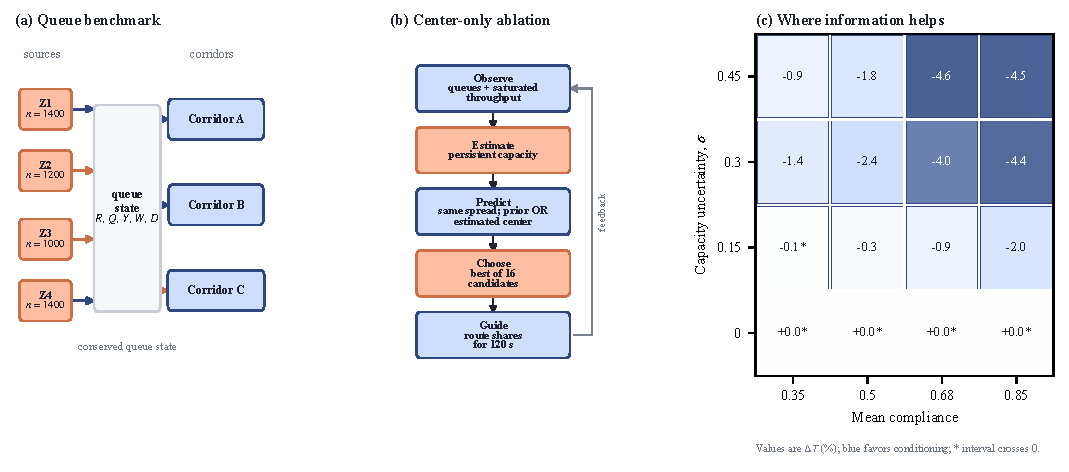
\includegraphics[width=0.90\textwidth]{fig1_system_overview.pdf}
    \caption{Benchmark and value-of-information design. (a) Base queue network. (b) Matched feedback controller. (c) Conditioned-minus-unconditioned mean clearance effect across uncertainty and compliance; negative values favor conditioning.}
    \label{fig:overview}
\end{figure*}

\section{Model and Online Information}
Let $\mathcal Z$ denote source zones and $\mathcal E$ destination corridors. The conserved state contains unreleased populations $R_z$, path queues $Q_{ze}$, travel-delay cells $Y^k_{ze}$, exit queues $W_e$, and cumulative discharge $D$. Recommendations $u_{ze}(t)$ mix with one-hot habitual routing $h_{ze}$ through compliance $\rho_z$:
\begin{equation}
p_{ze}(t)=\rho_z u_{ze}(t)+(1-\rho_z)h_{ze},\qquad \sum_e p_{ze}(t)=1.
\label{eq:compliance}
\end{equation}
For nominal path capacity $c_{ze}$, exit capacity $C_e$, and fixed multipliers $\xi_{ze},\zeta_e$,
\begin{align}
\widetilde Q_{ze}(t)&=Q_{ze}(t)+b_z(t)p_{ze}(t),\\
x_{ze}(t)&=\min\{\widetilde Q_{ze}(t),c_{ze}\xi_{ze}\Delta t\},\\
y_e(t)&=\min\{W'_e(t),C_e\zeta_e\Delta t\}.
\label{eq:flows}
\end{align}
Here $b_z(t)$ is released population during the step and $W'_e(t)$ includes arrivals from existing travel cells. Existing delay cells shift before newly admitted path flow enters the final delay cell, so new flow cannot reach an exit in the same step. Queue and discharge updates conserve total population; clearance occurs when active mass falls below $10^{-8}$ persons.

For $m_j\in\{\xi_{ze},\zeta_e\}$,
\begin{align}
\log \widetilde m_j&\sim\mathcal N(-\sigma^2/2,\sigma^2),\quad
m_j=\operatorname{clip}_{[0.45,1.35]}(\widetilde m_j),\\
\widetilde\rho_z&\sim\operatorname{Beta}(\mu\kappa,(1-\mu)\kappa),\quad
\rho_z=\operatorname{clip}_{[0.02,0.98]}(\widetilde\rho_z),
\label{eq:uncertainty}
\end{align}
with default $\mu=0.68$ and $\kappa=18$. All queue states are observed. A capacity estimate updates only when demand saturates the corresponding path or exit:
\begin{equation}
\widehat m(t+1)=(1-a)\widehat m(t)+a\frac{x(t)}{c\Delta t},\qquad a=0.3.
\label{eq:estimate}
\end{equation}
Saturation is classified using demand and the true step capacity in the simulator. Under this favorable, noise-free observation model, a saturated throughput identifies the true multiplier before smoothing. After $k$ saturated observations,
\begin{equation}
\widehat m_k-m=(1-a)^k(\widehat m_0-m).
\label{eq:convergence}
\end{equation}
An unsaturated observation instead supplies a lower bound on capacity: serving all demand $D$ implies $c m\Delta t\geq D$. It does not point-identify $m$, and the present estimator leaves its estimate unchanged. Estimator accuracy must therefore be interpreted jointly with saturation coverage; accurate bottleneck estimates need not imply identification of every link.

\section{Guidance and Evaluation}
The reactive baseline assigns route shares using free-flow time and current path/exit workload. Rolling-horizon policies use the same 16-candidate construction: habitual and reactive recommendations, mixtures of the reactive recommendation with equal shares, capacity--travel-time shares or the previous recommendation, and Dirichlet perturbations. Each candidate recommendation is held fixed during its eight-scenario, 300-s rollout. For terminally corrected clearance estimate $\widehat T_s$, mean person time $\bar A_s$, and peak queue-density proxy $d_s$, the score is
\begin{align}
L_s(u)&=\widehat T_s(u)+w_A\bar A_s(u)+w_d[d_s(u)-d_0]_+^2,\\
J(u)&=S^{-1}\sum_s L_s(u)+\lambda\CVaR_{0.8}(L(u))\notag\\
&\quad+w_s\operatorname{mean}_{z,e}|u_{ze}-u^{\rm prev}_{ze}|.
\label{eq:objective}
\end{align}
Clearance and mean person time are measured in minutes. The default weights are $w_A=0.25$, $w_d=6$ and $w_s=0.08$, with density threshold $d_0=3.5$; the primary policies set $\lambda=0$. The clearance surrogate adds terminal path work, exit work, and free-flow time to the simulated horizon; it is an approximation, not an exact remaining clearance time. The oracle uses the realized capacities with zero capacity-scenario spread, so its difference from conditioning also includes this change in dispersion.

Observation, candidate, and scenario substreams are derived independently at each control update, preventing state-dependent candidate sampling from shifting the scenario stream. The primary scenario coupling is explicit. For the same standard-normal draw $\varepsilon_j^s$ and the same compliance draw in scenario $s$,
\begin{align}
m_{\uncond,j}^s&=\operatorname{clip}\!\left(\exp[-\sigma^2/2+\sigma\varepsilon_j^s]\right),\\
m_{\cond,j}^s&=\operatorname{clip}\!\left(\widehat m_j\exp[-\sigma^2/2+\sigma\varepsilon_j^s]\right).
\label{eq:center-only}
\end{align}
Thus the center changes while the pre-clipping log-spread parameter, clipping rule, and random variates remain fixed. A secondary contracted-spread policy uses $\max(0.05,0.45\sigma)$ solely to quantify that separate design choice.

The base benchmark has 5000 people, four zones, and three corridors. Controllers update every 120~s with default $\Delta t=10$~s. The archived primary validation uses seeds 100000--100199 and 5000 paired-bootstrap resamples. Environment and policy seeds are separate; matched policies share each run's realized capacities and compliance. The frozen CSV tables are the numerical source for this revision. Diagnostic protocols use 50 seeds per uncertainty--compliance cell, 30 per time step, 50 per estimator regime, 50 per network family, and 30 per sensor regime. The time-step sweep holds the control interval, rollout horizon, and estimator decay in physical time fixed. Structural transfer covers the base network, symmetric, path-bottleneck, exit-bottleneck, and expanded 5-zone/4-corridor configurations at $\sigma=0.30$ and $\mu=0.68$. Controller-facing estimate faults include multiplicative log-noise 0.15, 60-s delay, 20\% dropout, and $+10\%$ bias. These modify the already-computed estimates passed to the controller; queue states, raw throughput and saturation classification remain ideal. They are evaluated in the default $(0.22,0.68)$ and high-information $(0.45,0.85)$ $(\sigma,\mu)$ regimes.

\subsection{Independent Same-State Diagnostics}
The additional diagnostic protocol uses 30 previously unused environmental seeds, 110000--110029, with policy seed equal to environmental seed plus 1000003. Both primary mean policies collect pre-decision states at 120, 360, and 600~s, giving at most 180 snapshots. A state already cleared at a sampling time is recorded as skipped and is not replaced. Saved states retain all queues, transit, estimator histories, previous recommendations, accumulated person time, and pre-decision policy/RNG state. Trace collection reuses the actual decision evaluation without consuming additional random draws.

At each snapshot, the selected and reactive recommendations are compared under the same realized capacities and compliance. One continuation holds each recommendation fixed to clearance. The other applies it for 120~s and then uses reactive guidance, recomputed every 120~s on that branch's own state. Outcomes are residual times from the snapshot; the absolute 3600-s limit is retained and incomplete branches are flagged. Equivalent recommendations count as reactive choices. We log full-objective gaps separately from clearance-component gaps, and compare the latter with realized fixed-action clearance ordering. The common-reactive continuation measures consequences of the current action; it is not a comparison of complete RH and reactive policies. Intervals use 5000 seed-cluster bootstrap resamples, retaining dependence among phases and trajectories from each environment.

Runtime uses the first five diagnostic seeds and the same eligible snapshots. Reactive, unconditioned mean, and conditioned mean decisions are measured serially, with one BLAS thread, five warmups and 30 timed repetitions per policy and snapshot. Every repetition resets state, policy and RNG; cloning, construction and file I/O are excluded. Cyclic measurement order reduces order effects. We report median and 95th-percentile decision times with hardware and software metadata.

\begin{table}[t]
\caption{Primary Paired Validation ($n=200$)}
\label{tab:final}
\centering
\footnotesize
\setlength{\tabcolsep}{3.0pt}
\begin{tabular}{lrrr}
\toprule
Policy & Mean & P90 & Mean peak\\
& (s) & (s) & (p/m$^2$)\\
\midrule
Static nearest & \StaticMean & \StaticPninety & \StaticDensity\\
Reactive balance & \ReactiveMean & \ReactivePninety & \ReactiveDensity\\
Unconditioned mean & \UncondMean & \UncondPninety & \UncondDensity\\
Conditioned mean & \CondMean & \CondPninety & \CondDensity\\
Oracle-capacity mean & \OracleMean & \OraclePninety & \OracleDensity\\
\bottomrule
\end{tabular}
\end{table}

\begin{figure*}[t]
    \centering
    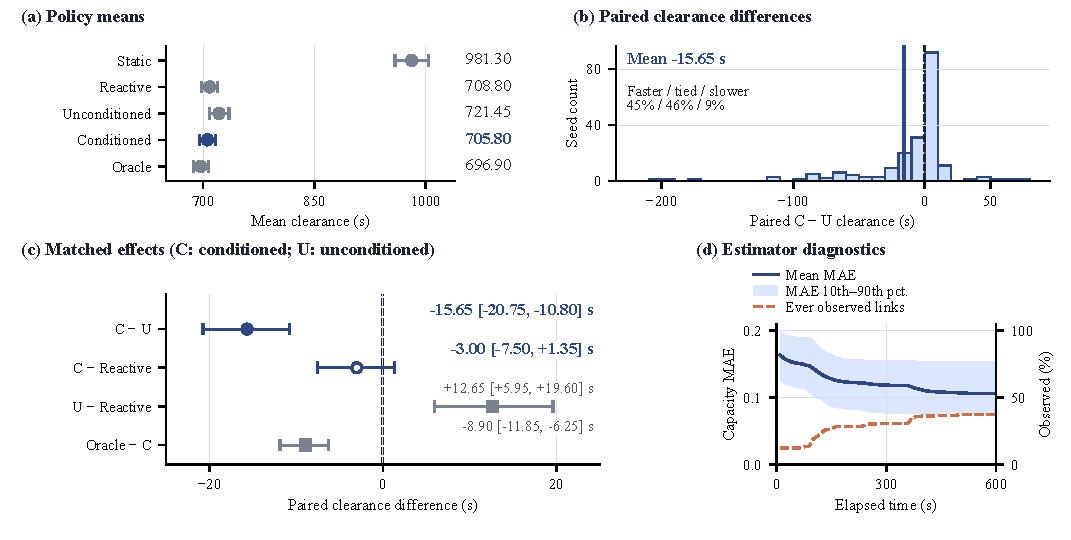
\includegraphics[width=0.90\textwidth]{fig2_performance_landscape.pdf}
    \caption{Primary evidence. (a) Paired-validation policy ladder. (b) Paired center-only information effect. (c) Component effects and direct conditioned--reactive comparison. (d) Default-regime capacity-estimator MAE and fraction of links ever observed under saturation.}
    \label{fig:primary}
\end{figure*}

\section{Results}
\subsection{Primary Validation and Observability}
Reactive balancing improved substantially over static routing (\DynamicDiff~s, 95\% interval $[\DynamicCILow,\DynamicCIHigh]$), whereas unconditioned lookahead differed from reactive control by \PlanningDiff~s ($[\PlanningCILow,\PlanningCIHigh]$). The center-only comparison averaged \CondMean~s versus \UncondMean~s, giving $\Delta T_{\rm sense}=\PrimaryDiff$~s (\PrimaryPct\%; $[\PrimaryCILow,\PrimaryCIHigh]$). The difference between marginal P90 values was \PrimaryPninetyDiff~s ($[\PrimaryPninetyCILow,\PrimaryPninetyCIHigh]$); win/tie/loss was \PrimaryWin\%/\PrimaryTie\%/\PrimaryLoss\%, and the worst observed paired harm was \WorstHarm~s. The direct conditioned-minus-reactive effect was \SystemDiff~s ($[\SystemCILow,\SystemCIHigh]$), about 0.42\% of the reactive mean. Its interval includes zero. The main 2.17\% benefit therefore describes improvement over unconditioned RH, not an established advantage over reactive guidance. The oracle was \OracleGapReduction~s faster than conditioned control (oracle-minus-conditioned interval $[\OracleGapCILow,\OracleGapCIHigh]$~s); zero spread, finite candidates, and finite lookahead limit its interpretation.

The contracted-spread diagnostic changed clearance by \SpreadDiff~s relative to the equal-spread conditioned controller ($[\SpreadCILow,\SpreadCIHigh]$). This separates any benefit from narrowing the scenario distribution from the primary value of moving its center.

Figure~\ref{fig:primary}(d) reports the information mechanism directly. In the default regime, combined capacity-multiplier MAE changed from \EstimatorInitialMAE{} at the first recorded step to \EstimatorMAETwoForty{} at 240~s, when \EstimatorObservedTwoForty\% of links had been observed under saturation. At clearance, mean MAE was \EstimatorFinalMAE{} and mean observed fraction was \EstimatorFinalObserved\%. At clearance, path MAE was \PathFinalMAE{} with \PathObservedPct\% of paths ever observed saturated; exit MAE was \ExitFinalMAE{} with \ExitObservedPct\% coverage. This pattern is consistent with informative exit bottlenecks, but does not isolate their causal contribution without path-only/exit-only ablations. These are benchmark diagnostics rather than field-sensor accuracy claims.

\subsection{Operating Regions and Robustness}
The map in Fig.~\ref{fig:overview}(c) shows that information becomes actionable jointly through uncertainty and compliance. At $\sigma=0.45$, conditioned-minus-unconditioned effects across $\mu\in\{0.35,0.50,0.68,0.85\}$ were \MapHighCThreeFive, \MapHighCFiveZero, \MapHighCSixEight, and \MapHighCEightFive~s, respectively. At negligible uncertainty, effects were correspondingly small or unresolved. Because each map cell is diagnostic and not multiplicity-adjusted, the map supports regional patterns rather than cell-level guarantees.

\begin{figure*}[t]
    \centering
    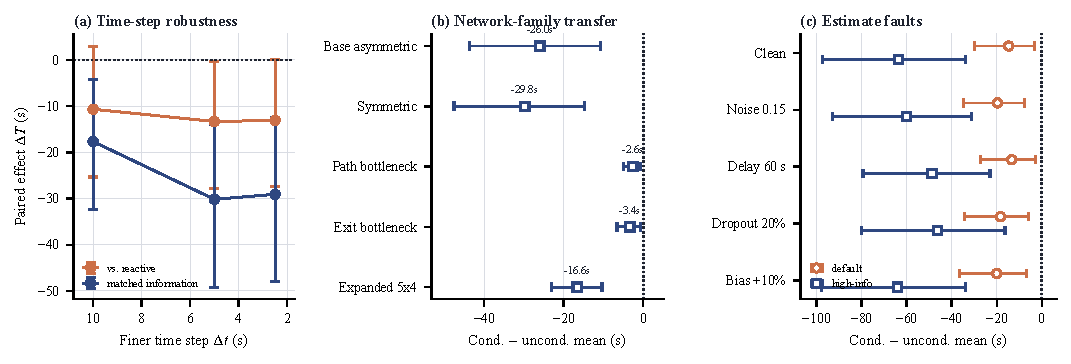
\includegraphics[width=0.90\textwidth]{fig3_context_validation.pdf}
    \caption{Transfer and failure diagnostics. (a) Time-step robustness. (b) Center-only effects across five synthetic network families at $\sigma=0.30$ and $\mu=0.68$. (c) Controller-facing estimate-fault effects in the default and high-information regimes. Intervals are paired-bootstrap 95\% intervals.}
    \label{fig:robustness}
\end{figure*}

The matched effect was \TimeTen, \TimeFive, and \TimeTwoFive~s at time steps of 10, 5, and 2.5~s, respectively. Across the five network families, \TopologyResolvedCount{} of \TopologyCount{} effects had intervals entirely below zero; point estimates ranged from \TopologyBest{} to \TopologyWorst~s. The network study varies structural bottlenecks and size, but remains synthetic.

Under clean controller-facing estimates, the effect was \DefaultCleanSensor~s in the default regime and \HighInfoCleanSensor~s in the high-information regime. Across the four faults, estimates ranged from \DefaultFaultLow{} to \DefaultFaultHigh~s and from \HighInfoFaultLow{} to \HighInfoFaultHigh~s, with every interval below zero. At high information, delay and dropout attenuated the clean point estimate, whereas noise and bias were nonmonotone. These checks test errors in the estimates delivered to control, not the complete raw-sensing and saturation-classification pipeline.

\subsection{Candidate Selection and Computation}
\DiagnosticResultsText

\begin{figure*}[t]
    \centering
    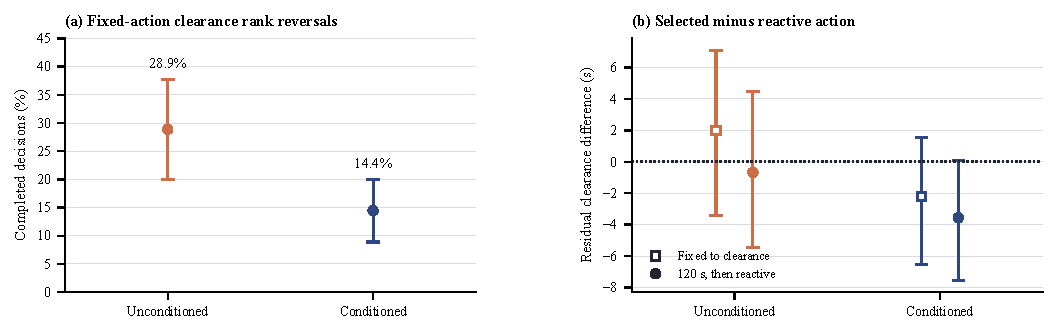
\includegraphics[width=0.90\textwidth]{fig4_decision_diagnostics.pdf}
    \caption{Independent same-state decision diagnostics. (a) Strict reversals between predicted clearance-component and realized fixed-action ordering, as a percentage of all 90 completed decisions per collector; predicted or actual ties are not reversals. (b) Mean selected-minus-reactive residual clearance differences under both continuations; negative values favor the selected action. Intervals are 95\% seed-bootstrap intervals.}
    \label{fig:decisions}
\end{figure*}

\begin{table}[t]
\caption{Decision Runtime on Shared Diagnostic States}
\label{tab:runtime}
\centering
\footnotesize
\begin{tabular}{lrr}
\toprule
Controller & Median (ms) & p95 (ms) \\
\midrule
Reactive & 0.021 & 0.039 \\
Unconditioned mean & 4.050 & 4.590 \\
Conditioned mean & 4.042 & 4.515 \\
\bottomrule
\end{tabular}

\end{table}
\RuntimeResultsText

\section{Discussion}
The center-only design supports an internal causal interpretation within the implemented benchmark: the programmed intervention changes the location of the capacity predictions, not their log-spread parameter, clipping rule, candidate architecture, objective, or scenario random draws. The subsequent divergence in states and selected actions is an endogenous consequence of that intervention rather than an additional experimental change. The operating map shows that the benefit depends on uncertainty and compliance in the tested configurations. The observability summaries are consistent with information about bottlenecks being useful; identifying which links drive the effect would require additional ablations.

External validity remains the principal limitation. The simulator omits continuous pedestrian interaction, group behavior, detailed geometry, counterflow, collision avoidance, pressure, smoke, and injury risk. Saturated throughput is deliberately informative, all queue states are available, and the network families are designed rather than empirically calibrated. Real systems would require saturation-classification error, aggregation, privacy, latency, missing-data, change detection, venue calibration, and professional safety review \cite{shi2018state}. At high $\sigma$, clipping shifts the realized environmental mean; reported effects use that clipped distribution. A shifted center near a bound can also change post-clipping moments, although both controllers apply the same transform. The EWMA already discounts older observations. Tracking an abrupt capacity change would nevertheless depend on obtaining new saturated observations and on estimation and control update times; incident tracking and change detection require separate validation.

The inclusion of a reactive candidate does not guarantee that RH clears faster than the reactive policy. A candidate is held constant for 300~s in prediction, whereas the executed reactive policy recomputes its recommendation every 120~s. Moreover, minimizing Eq.~\eqref{eq:objective} need not minimize realized final clearance: the objective also values person time, density and switching. Nominal capacity centers, finite scenario samples and the terminal approximation can alter the ranking. These explain the absence of a guarantee. The nonzero fixed-action rank-reversal rates document disagreement between the clearance surrogate and realized fixed-action ordering. However, the mean effects in both counterfactual continuations have intervals that include zero. The diagnostics neither establish a selected-action clearance advantage nor apportion the full-policy difference among capacity centers, finite scenario sampling, terminal approximation and objective trade-offs.

The primary benefit is modest: the final clearance instant is earlier by about 16~s in a roughly 12-min process, not a 16-s saving for every person. The paired median is zero and some runs are slower. For an existing RH system with usable throughput data, the within-controller comparison is relevant to adding capacity estimation. For a system currently using reactive guidance, the direct comparison is the relevant adoption evidence and remains unresolved here. Runtime quantifies computation on the measured machine; instrumentation, calibration, maintenance and deployment costs are unmeasured. Neither these timings nor the queue-density proxy establish an operational safety gain.

\section{Conclusion}
Updating persistent-capacity forecast centers improved mean clearance within the specified RH benchmark by \PrimaryReduction~s (\PrimaryReductionPct\%). The direct advantage over reactive guidance remains unresolved. The matched comparison, observability summaries and independent decision diagnostics separate a within-controller information benefit from a general claim for predictive guidance. The conclusions concern synthetic fixed-capacity networks with ideal state observations; raw-sensor faults, abrupt incidents and venue-calibrated performance remain unvalidated.

\section*{AI Assistance Disclosure}
Generative AI tools assisted manuscript revision and research-code development. Responsibility for the final manuscript, code, and interpretation remains with the authors.

\IEEEtriggeratref{6}
\bibliographystyle{IEEEtran}
\bibliography{references}

\end{document}
